\section{需求基础}

\subsection{需求的定义}
IEEE的需求定义:
\begin{enumerate}[label=(\arabic*)]
    \item 用户为了解决问题或达到某些目标所需要的条件或能力;
    \item 系统或系统部件为了满足合同、标准、规范或其它正式文档所规定的要求而需要具备的条件或能力;
    \item 对(1)或(2)中的一个条件或一种能力的一种文档化表述。
\end{enumerate}

\subsection{基本概念区分}

\subsubsection{问题域}
\begin{itemize}
    \item 问题的产生地:当现实的状况与人们期望的状况产生差距时,就产生了问题。
    \item 要解决问题,就需要改变现实当中某些实体的状态或改变实体状态变化的演进顺序,使其达到期望的状态或演进顺序。
    \item 这些实体和状态构成了问题解决的基本范围,称为该问题的问题域。
\end{itemize}

\subsubsection{解系统}
软件系统通过影响问题域,能够帮助人们解决问题,称之为解系统
\begin{itemize}
    \item 问题域是自治的,它有自己的运行规律,而且这些规律不会因解系统的引入而发生改变
    \item 用户应关注问题域,\textbf{开发者应以问题域为中心思考}
\end{itemize}

\subsubsection{软件解决问题的基础:模拟与共享}
软件系统能够与问题域进行交互和相互影响的原因在于\textbf{软件系统中的某些部分对问题域中的某些部分的具有模拟特性}
\begin{itemize}
    \item 软件系统当中含有问题域某些部分的模型(或模拟),常见的模型包括数据模型、对象模型、处理模型等
    \item 问题域中的某些信息能够和模型中的信息建立映射关系
\end{itemize}
 
这些通过映射建立的共同知识,就是问题域和解系统之间的共享现象
\begin{itemize}
    \item 共享现象就是解 系统所模拟的问题域部分,该部分在两个系统中同时存在
    \item 除了共享现象之外, 同题城还有一些没有被解系统模拟的知识,因为现实世界非常复杂,不可能也没必要在解系统中完全重现 
\end{itemize}
\begin{figure}[H]
	\centering
	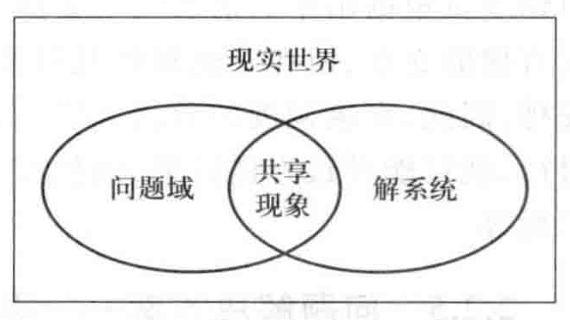
\includegraphics[width=0.3\textwidth]{img/问题域和解系统的关系.png}
\end{figure}

\subsubsection{问题域的特性}
问题域自治的规律性称为问题域特性
\begin{itemize}
    \item 问题域是自治的,它有自己的运行规律,而且这些规律不会因解系统的引入而发生改变
\end{itemize}

需额外关注的问题域特性
\begin{itemize}
    \item 间接特性
    \item 约束和假设 
    \begin{itemize}
        \item 社会性因素
    \end{itemize}
\end{itemize}

问题域特性的重要性
\begin{itemize}
    \item 要想解决问题,它就需要了解问题域特性,将解决方案和问题域特性结合起来 
    \item 要防止解系统的引入在问题域当中引发未预见的连锁反应 (例:间接特性不直接与解系统交互而引发)
\end{itemize}

\subsubsection{解系统的特性}
\begin{itemize}
    \item 解系统是问题的解决手段,并不是问题的产生地,所以解系统并不是问题域的一部分。解系统与问题域之间存在可以互相影响的接口,以实现交互活动。
    \item 用户不应该关注软件系统,而是关注问题。
    \item 开发者关注软件系统,但要学会以问题为中心思考。
\end{itemize}


\begin{figure}[H]
	\centering
	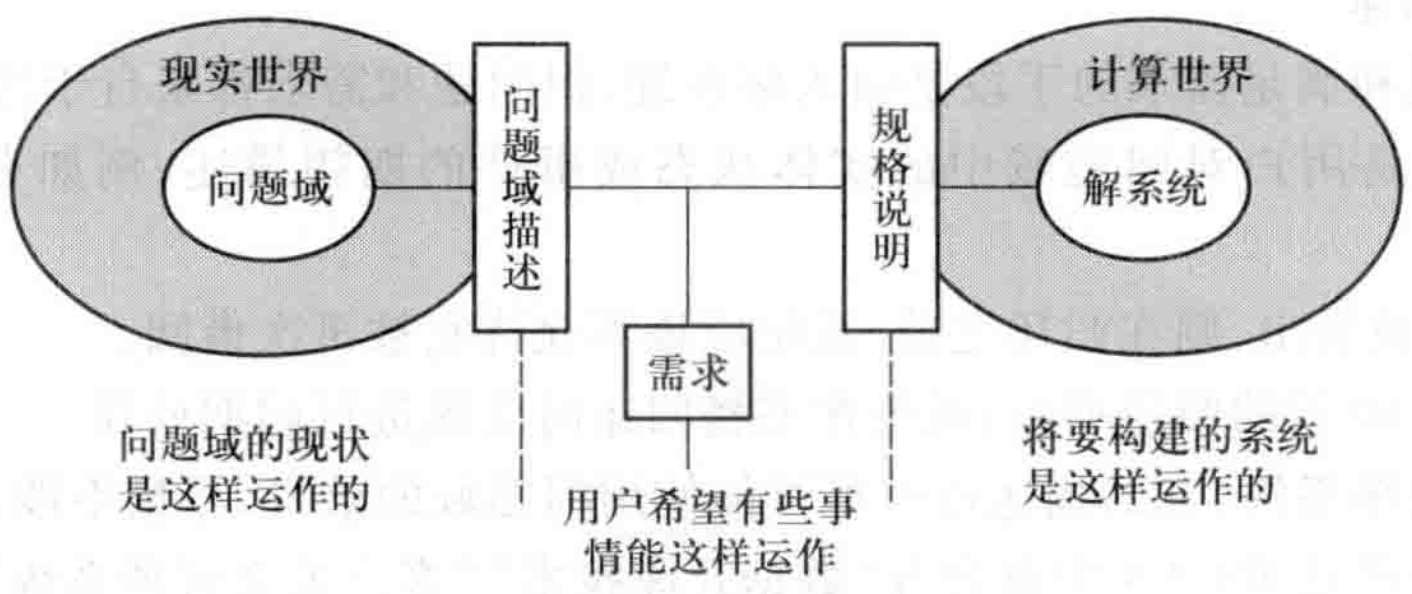
\includegraphics[width=0.55\textwidth]{img/问题域、需求、解系统、需求规格说明关系示意图.png}
\end{figure}

\subsubsection{需求规格说明}
因为解决方案以对外交互的方式定义了软件系统的功能,所以解决方案被称为软件系统的需求规格说明

IEEE将需求规格说明定义为:规定系统或部件的需求的文档,典型地包括功能需求、性能需求、接口需求、设计需求和开发标准。

\subsubsection{需求开发的形式化定义}
描述明确的问题域特性$E$,定义良好的系统行为$S$,预期的需求$R$
\begin{itemize}
    \item 需求工程的目的就是根据$E$,构建$S$,使得$E,S\mapsto R$
    \item 需求工程的困难之处:
    \begin{itemize}
        \item 不存在描述明确的$E$
        \item 不存在确定的针对$S$的评估标准$R$;
        \item $E,S \Rightarrow R$是一个创造性的过程。
    \end{itemize}
    \item 需求工程的主要工作:
    \begin{itemize}
        \item 需求开发,确定$R$
        \item 研究问题背景,描述问题域特性$E$
        \item 构建解系统,描述解系统行为$S$,使得$E,S\mapsto R$
    \end{itemize}
\end{itemize}

\subsubsection{需求工程的基本活动与实质}
\begin{figure}[H]
	\centering
	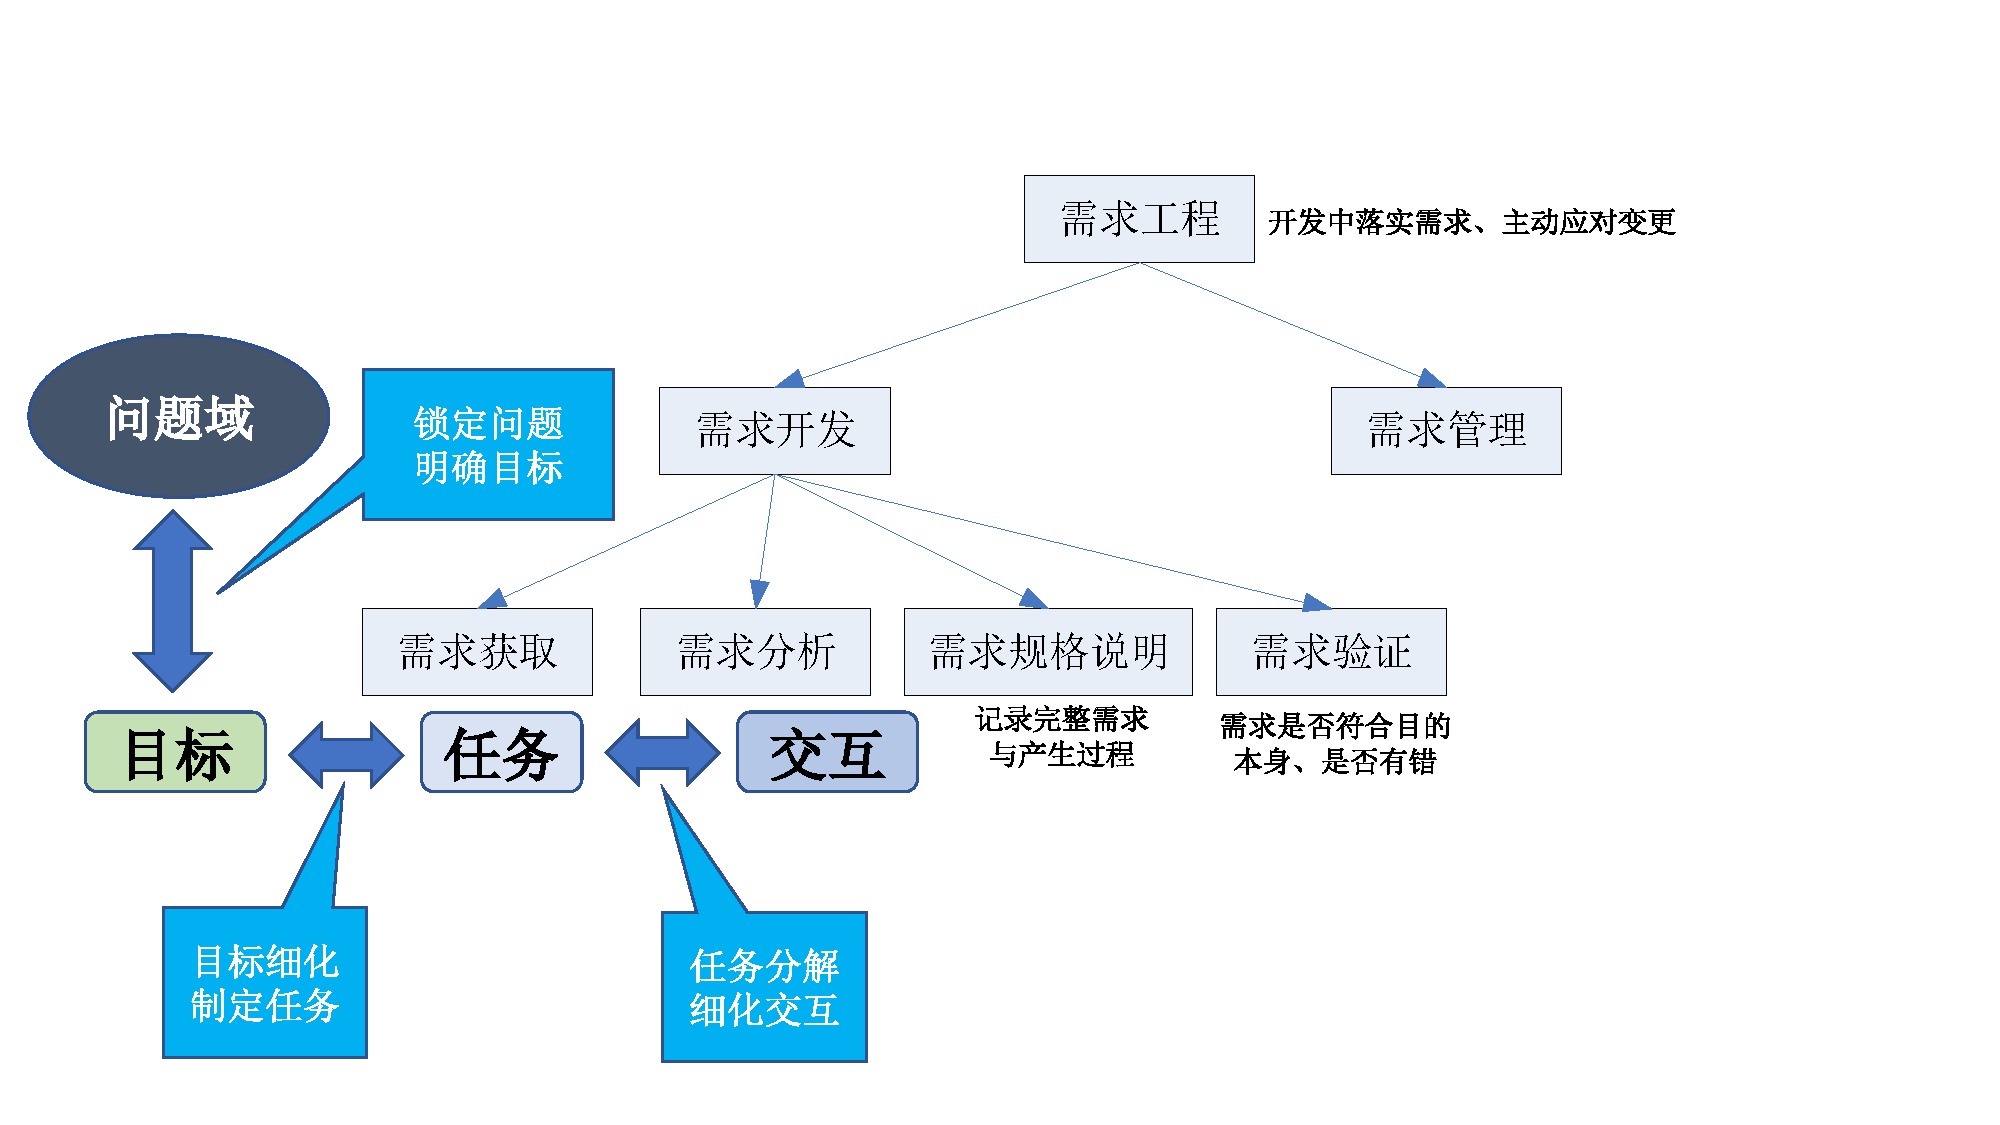
\includegraphics[width=0.8\textwidth]{img/需求工程的基本活动与实质.pdf}
\end{figure}

\subsubsection{需求工程活动的困难性}
\begin{itemize}
    \item 问题域、目标、任务、交互的相互转化是创造性的活动
    \begin{itemize}
        \item 每个案例都有其独特性,不可复用,接近于艺术
        \item 需要对问题所在的领域有着深刻的认识
        \item 需要掌握一套设计思维与辅助工具,并多多练习
    \end{itemize}
    \item 编程与设计方面的能力不能直接用于需求分析 
    \begin{itemize}
        \item 设计和编程都有构建高质量软件的共同目标,而且使用相同的概念和组织机制保证了从设计到编程的平滑过渡,所以,结构化与面向对象思维在设计领域也取得了成功
        \item 但是需求分析除了拥有构建高质量软件的目标之外,还有一个更加重要的目标是理解现实中的非技术性和社会性因素
    \end{itemize}
    \item 文档撰写、功能验证、基线管理需要丰富的开发与管理经验
\end{itemize}


\subsubsection{需求工程师:现实世界方面与技术方面的桥梁}
好的需求工程师更应该扮演好涉众代理的角色,站在涉众的立场想问题,替涉众跟踪和监控软件开发过程,保护涉众的利益
\begin{figure}[H]
	\centering
	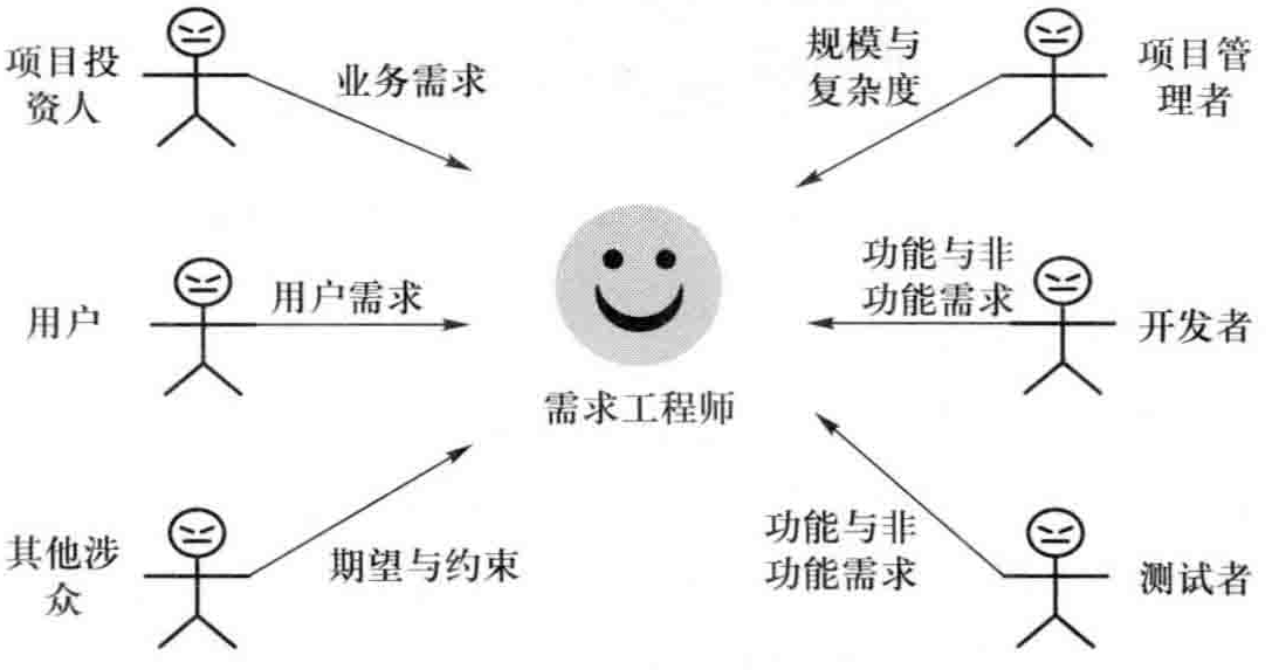
\includegraphics[width=0.6\textwidth]{img/需求工程师的桥梁作用.png}
\end{figure}

需求工程师需要具备的技能
\begin{figure}[H]
	\centering
	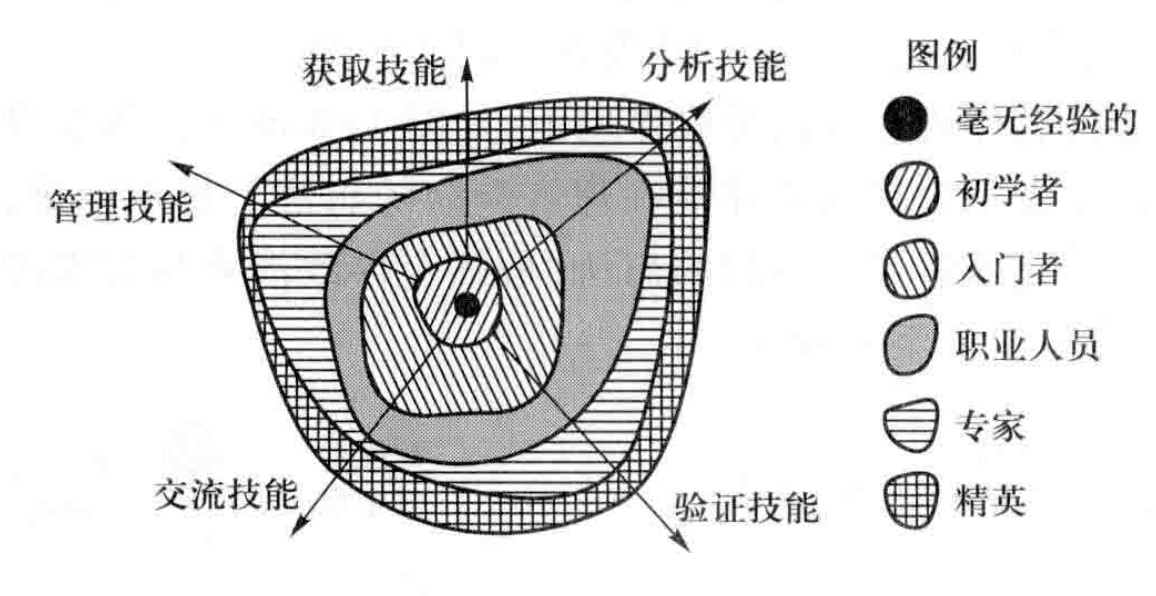
\includegraphics[width=0.55\textwidth]{img/需求工程师需要具备的技能.png}
\end{figure}

\subsection{需求的层次性}












